\documentclass{article}

\usepackage{amsmath}
\usepackage{xcolor,listings}
\usepackage{graphicx}

\title{Group Project 2\\Problem 1}
\author{Group 26\\JJ (John) Brown, David Jones,\\Charlie (Charles) Ruiter, Stephanie Whitworth}
\date{Due 2018-10-01}

\renewcommand{\thesubsection}{\alph{subsection}}
% \renewcommand{\thesection}{Problem {section}} % note done yet -- want like "Problem 1"

\begin{document}
\maketitle

\section{}
\subsection{Write a description for the attached ER diagram}

\begin{itemize}
\item A passenger has a unique ID number and a name consisting of a first and last name. They also have multiple email addresses.
\item An employee has a unique SSN, a name consisting of a first and last name, a date they were hired, and a dynamically-computed number of years of service.
\item An employee may train another employee. Each employee only trains one trainee, and each trainee has only one trainer.
\item There are two mutually-exlusive kinds of employees: a driver, and a mechanic.
\item A driver has a licence, which has an id, class, and expiration date.
\item A mechanic has a certification, which has a type and a date.
\item Passengers can ride taxis. A taxi has a unique id number, a make, a model, and a year.
\item When a passenger rides a taxi, a record is kept of who rode, which taxi they rode, who the driver was, and the date they rode.
\item Every taxi parks overnight in a parking spot. Within a parking complex, a parking spot has a level and a spot number.
\item A parking complex has many parking spots, on various levels. Each parking spot in the same parking complex has a different spot number and level, but parking spots in different garages may have the same values for those fields.
\item A parking complex has a unique name, and a location. That location consists of a number, a street, a city, a state, and a ZIP.
\item When a mechanic services a taxi, a record is made of which mechanic serviced which taxi and the date it was serviced.
\item Finally, a driver may accept work from a mechanic. Every service is associated with a driver responsible for the service.
\end{itemize}

\subsection{Convert the attached ER diagram to a Relational Database}

\begin{lstlisting}[
	language=SQL,
	morekeywords={REFERENCES},
	breaklines=true,
    postbreak=\mbox{\textcolor{red}{$\hookrightarrow$}\space}, % https://tex.stackexchange.com/questions/116534/lstlisting-line-wrapping
    keywordstyle=\color{blue},
    stringstyle=\color{green},
	]
CREATE TABLE Passenger(
	Passenger_id NUMERIC,
	First_Name VARCHAR,
	Last_Name VARCHAR,
	PRIMARY KEY(Passenger_id)
);
CREATE TABLE Passenger_Email_Address(
	FOREIGN KEY Passenger(Passenger_id) Passenger_id,
	Email_Address VARCHAR
);
CREATE TABLE Employee(
	Employee_SSN NUMERIC,
	First_Name VARCHAR,
	Last_Name VARCHAR,
	Hire_Date DATE,
	Service_Years NUMERIC AS DATE_FORMAT( DATEDIFF( NOW(), Hire_Date), "%Y")+0,
	FOREIGN KEY (Trainer_SSN) REFERENCES Employee(Employee_SSN),
	PRIMARY KEY (Employee_SSN)
);

CREATE TABLE Driver(
	FOREIGN KEY (Employee_SSN) REFERENCES Employee(Employee_SSN),
	Licence_id NUMERIC,
	Licence_Class VARCHAR,
	Licence_Expiration DATE,
	PRIMARY KEY (Employee_SSN)
);

CREATE TABLE Mechanic(
	FOREIGN KEY (Employee_SSN) REFERENCES Employee(Employee_SSN),
	Certification_Type VARCHAR,
	Certification_Date DATE,
	PRIMARY KEY (Employee_SSN)
);

CREATE TABLE Taxi(
	Taxi_id NUMERIC,
	Make VARCHAR,
	Model VARCHAR,
	Year NUMERIC,
	FOREIGN KEY (Parking_Complex_Name, Parking_Spot_Number, Parking_Spot_Level) REFERENCES Parking_Spot(Parking_Complex_Name, Parking_Spot_Number, Parking_Spot_Level),
	PRIMARY KEY (Taxi_id)
);

CREATE TABLE Services(
	FOREIGN KEY (Taxi_id) REFERENCES Taxi(Taxi_id),
	FOREIGN KEY (Mechanic_SSN) REFERENCES Mechanic(Employee_SSN),
	Date DATE,
	FOREIGN_KEY (Accepting_Driver_SSN) REFERENCES Driver(Employee_SSN)
);

CREATE TABLE Ride(
	FOREIGN KEY (Passenger_id) REFERENCES Passenger(Passenger_id),
	FOREIGN KEY (Taxi_id) REFERENCES Taxi(Taxi_id),
	FOREIGN KEY (Driver_SSN) REFERENCES Driver(Employee_SSN)
);

CREATE TABLE Parking_Spot(
	FOREIGN KEY (Parking_Complex_Name) REFERENCES Parking_Complex(Parking_Complex_Name),
	Spot_Number NUMERIC,
	Level NUMERIC
	PRIMARY KEY (Parking_Complex_Name, Spot_Number, Level)
);

CREATE TABLE Parking_Complex(
	Parking_Complex_Name VARCHAR,
	Location_Number VARCHAR,
	Location_Street VARCHAR,
	Location_City VARCHAR,
	Location_State VARCHAR,
	Location_ZIP VARCHAR,
	PRIMARY KEY (Parking_Complex_Name)
);
\end{lstlisting}


\subsection{Draw a Schema Diagram for the relational database}

\begin{figure}[h!]
	
	\caption{Schema Diagram for Problem 1}
    
	\centering
        
	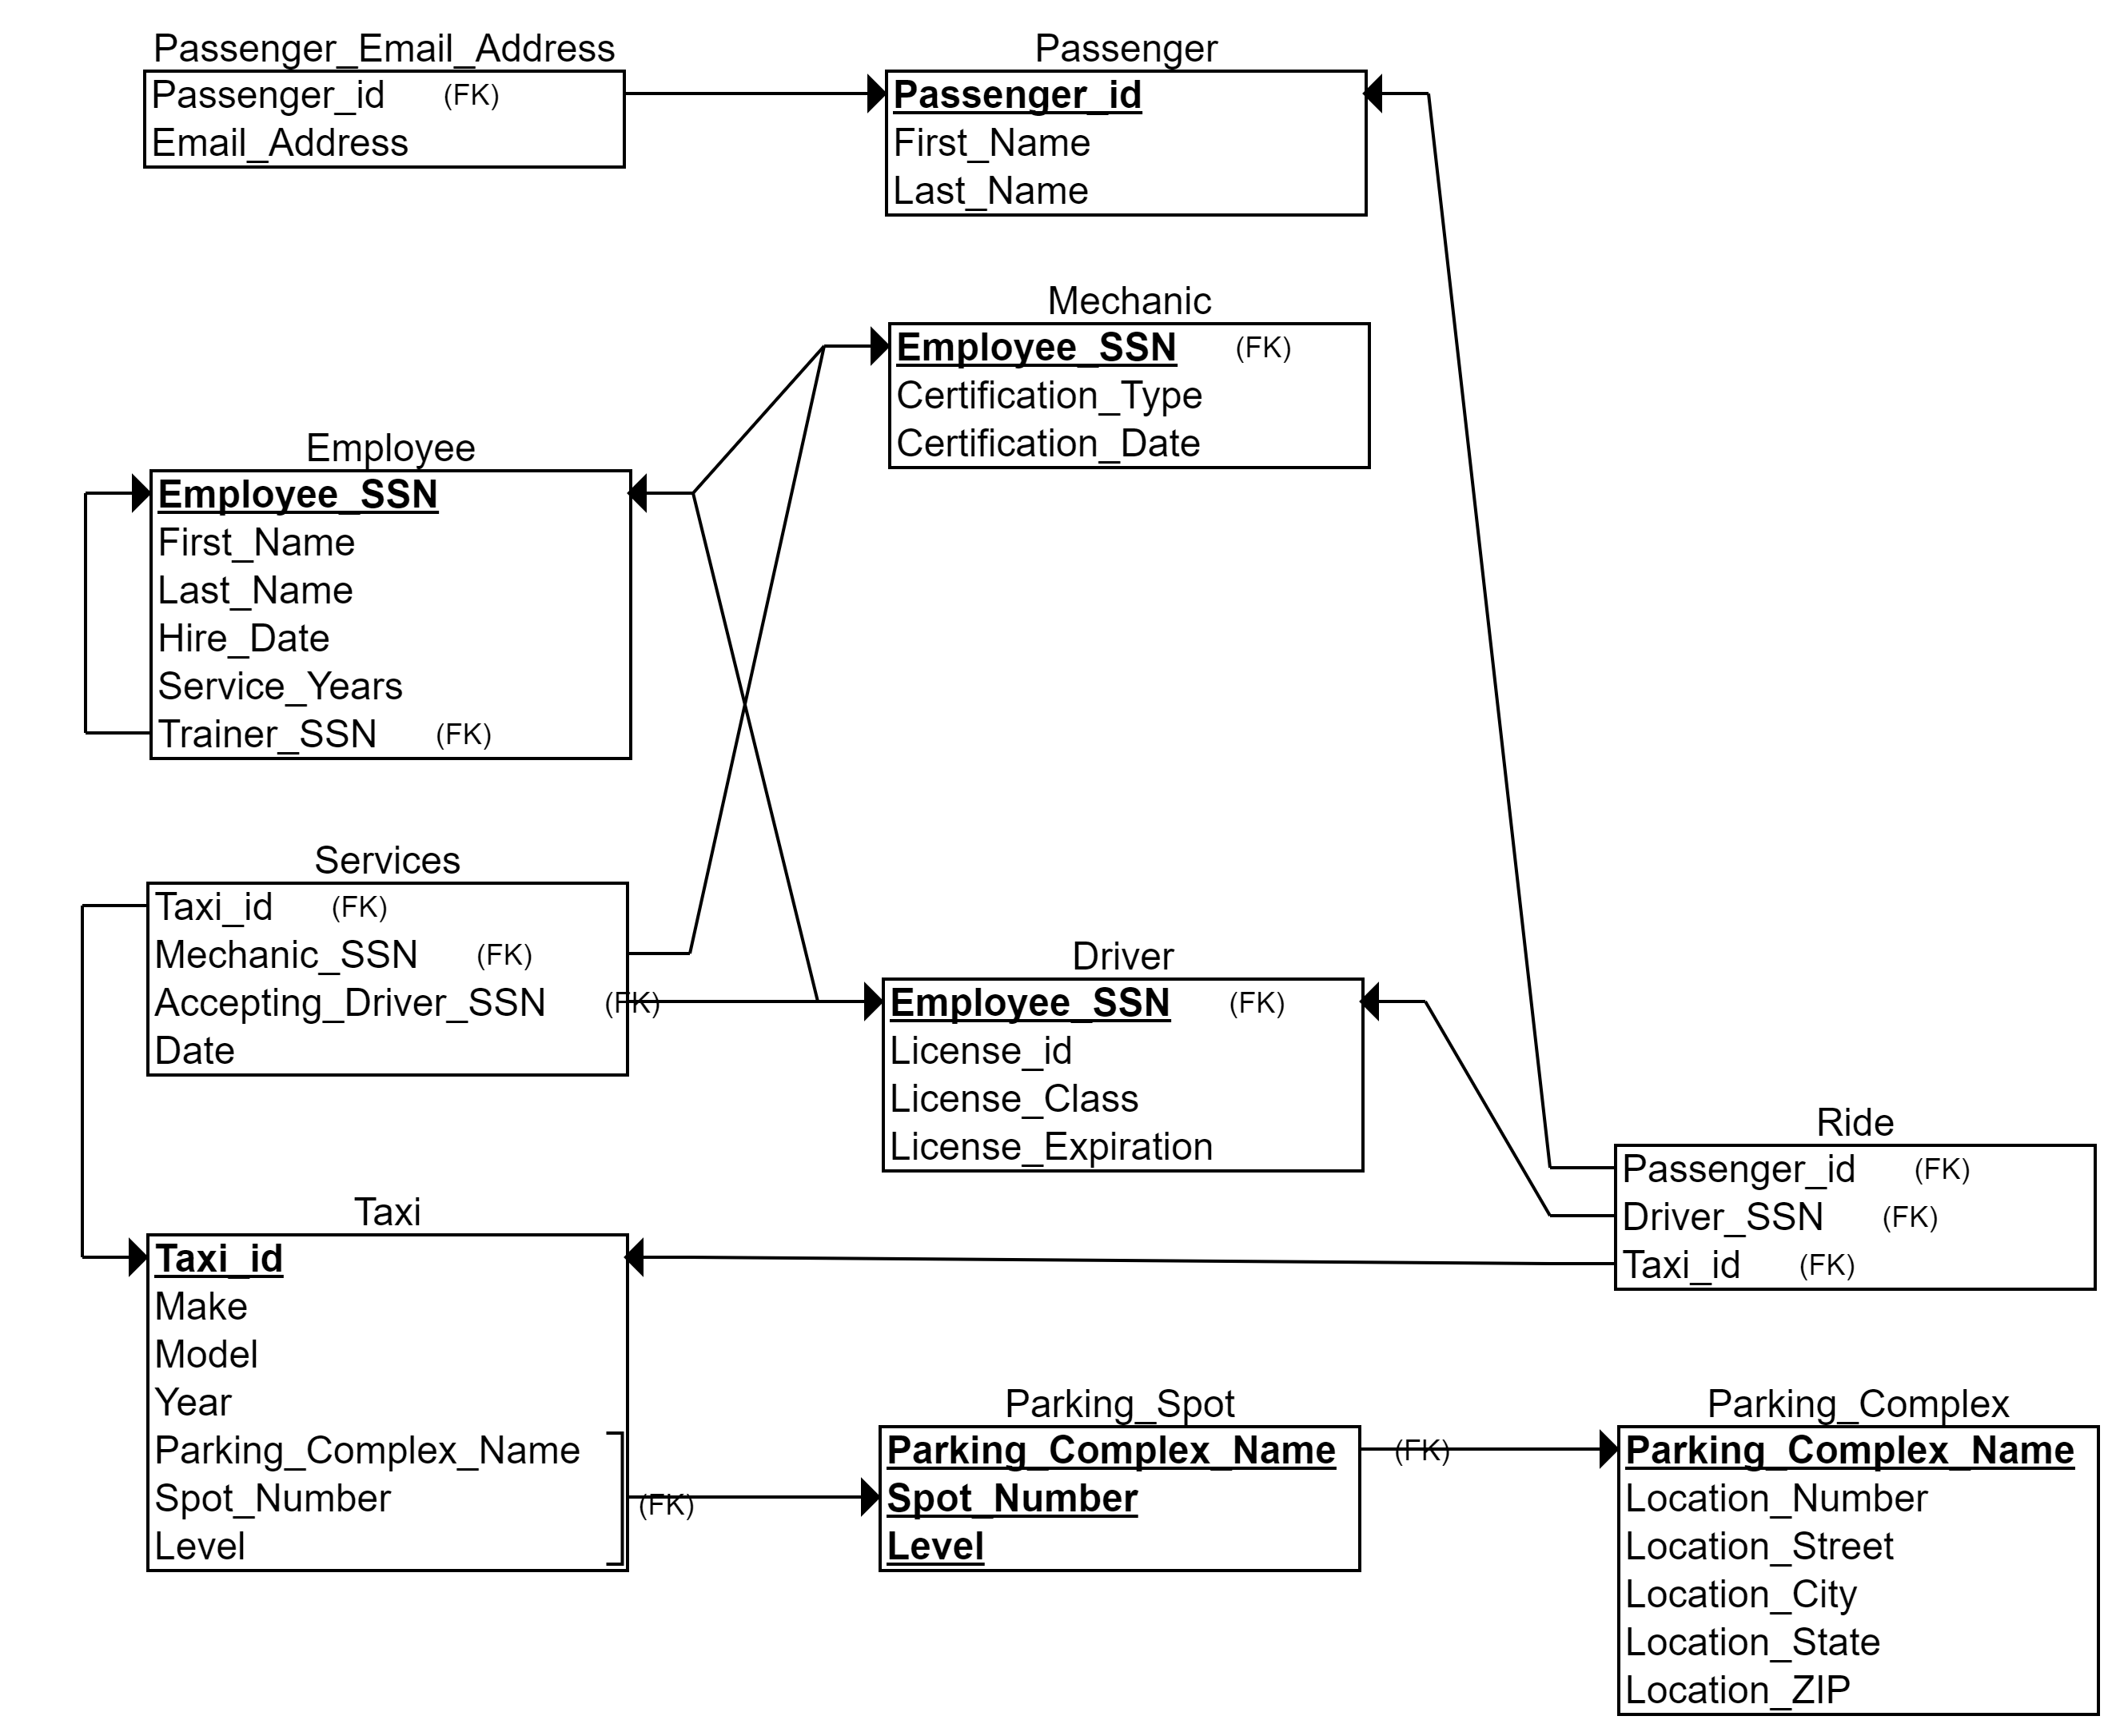
\includegraphics[width=\textwidth]{img/1c-figure.png}

\end{figure}

\end{document}
